% ______________________________________________________________________________
%
% DVG001 -- Introduktion till Linux och små nätverk
%                                     Projektarbete
% ~~~~~~~~~~~~~~~~~~~~~~~~~~~~~~~~~~~~~~~~~~~~~~~~~
% Author:   Jonas Sjöberg
%           tel12jsg@student.hig.se
%
% Date:     2016-06-07 -- 2016-06-13
%
% License:  Creative Commons Attribution 4.0 International (CC BY 4.0)
%           <http://creativecommons.org/licenses/by/4.0/legalcode>
%           See LICENSE.md for additional licensing information.
% ______________________________________________________________________________


% ______________________________________________________________________________
\section{Servern som lokal IPv6-router}
Debian-servern kan konfigureras för att agera router åt övriga datorer i det
lokala nätverket. På så vis kan de också göra IPv6-anslutningar.

Till att börja med ändrades filen \texttt{/etc/sysctl.conf}. 
Den ändrade raden visas i Programlistning~\ref{listing:sysctl}.

\configsource{include/conf_sysctl}
             {Utdrag ur konfigurationsfilen \texttt{/etc/sysctl.conf}.}
             {listing:sysctl}

\subsection{DMZ}
Det lokala nätverkets router ställs in att först skicka all trafik till
Debian-servern genom att \texttt{DMZ} aktiveras i routerns konfiguration genom
ett konfigurationsinterface som nås genom en webbläsare.  
Detta visas i Figur~\ref{fig:dmz}.

\begin{figure}[H]
  \centering
  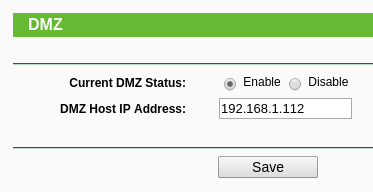
\includegraphics[width=0.5\linewidth]{include/dmz}
  \caption[Skärmdump på inställning av \texttt{dmz}]
          {Skärmdump på inställning av \texttt{dmz} i nätverkets router.}
  \label{fig:dmz}
\end{figure}


% ______________________________________________________________________________
\subsection{Konfigurationsfiler}
\subsubsection{\texttt{/etc/network/interfaces}}
Konfigurationsfilen \texttt{/etc/network/interfaces} har nu det slutgiltiga
utseendet i Programlistning~\ref{listing:interfaces-final}.

\configsource{include/conf_interfaces-final}
						 {Slutgiltigt innehåll i konfigurationsfilen
					    \texttt{/etc/network/interfaces}.}
             {listing:interfaces-final}


\subsubsection{\texttt{/etc/radvd.conf}}
Konfigurationsfilen \texttt{/etc/radvd.conf} får utseendet i
Programlistning~\ref{listing:radvd} för att Debian-servern ska fungera som
lokal IPv6-router.

\configsource{include/conf_radvd}
						 {Innehåll i konfigurationsfilen \texttt{/etc/radvd.conf}.}
             {listing:radvd}


\subsection{Brandvägg}
När servern börjat routa trafik från IPv6-tunneln till det lokala
nätverket får varje enhet på det lokala nätverket en egen publik IPv6-adress.
De lämnas då i ett mycket sårbart läge för eventuella intrång och det
är viktigt att en brandvägg skyddar dem. 

Direkt efter att Debian-servern blottas direkt mot internet görs upprepade
anslutningsförsök till \texttt{SSH}-servern från IP-adresser från området
\texttt{121.18.238.0/24}, vilket genom en uppslagning med kommandot
\texttt{whois} visade sig vara från Kina.

Då den enda vi förväntar oss ska ansluta till servern kommer från Sverige
kördes ett skript \cite{blockchina} som massblockerar adresser från bland annat
Kina och andra länder vi inte behöver släppa fram. Skriptet är helt enkelt en
lång lista av \texttt{ufw deny from ADRESS to any port 22} som körs i sekvens.

Inledningsvis användes \texttt{shorewall6} men efter upprepade misslyckanden
med konfigurationen övergavs \texttt{shorewall} för \texttt{ufw}.

Inställningar i brandväggen gjordes efter instruktioner från flera källor
\cite{ipv6:settingup} \cite{debian:networkconfig}
\cite{ipv6:tunnelswithdebian}.


\subsection{Test av routade IPv6-anslutningar}
Debian-servern förser enheter anslutna till det lokala nätverket med åtkomst av
IPv6-adresser genom tunneln. Vid testet ansluter maskiner i det lokala
nätverket till IPv6 genom Debian-serverns tunnel, till DNS-tjänsten dynv6 som 
i sin tur pekar mot den hemsida som Debian-servern hostar.  Detta
visas i Figur~\ref{fig:route1}, Figur~\ref{fig:route2}, Figur~\ref{fig:route3}
och Figur~\ref{fig:route4}.

\screenshot{include/08_ipv6routing_6465}
           {Skärmdump på test av routad IPv6-anslutning.}
           {Skärmdump på test av routad IPv6-anslutning genom Debian-servern, 
            till den hemsida som Debian-servern hostar genom DNS.
            Här från maskinen \texttt{ProBook-6465b}.}
           {fig:route1}

\screenshot{include/09_ipv6routing_probookii}
           {Skärmdump på test av routad IPv6-anslutning.}
           {Skärmdump på test av routad IPv6-anslutning genom Debian-servern,
            till den hemsida som Debian-servern hostar genom DNS.  Här från
            maskinen \texttt{ProBookII}.}
           {fig:route2}

\screenshot{include/10_ipv6routing_smartphone}
           {Skärmdump på test av routad IPv6-anslutning.}
           {Skärmdump på test av routad IPv6-anslutning genom Debian-servern,
            till den hemsida som Debian-servern hostar genom DNS.  Här från en
            \texttt{Samsung Galaxy S4} Android telefon.}
           {fig:route3}

\screenshot{include/11_ipv6routing_smartphone}
           {Skärmdump på test av routad IPv6-anslutning.}
           {Skärmdump på test av routad IPv6-anslutning genom Debian-servern,
            till den hemsida som Debian-servern hostar genom DNS.  Här från en
            \texttt{OnePlus X} Android telefon.}
           {fig:route4}


% ______________________________________________________________________________
\subsection{Routingmodell}
Nätverkets konfiguration illustreras i Figur~\ref{fig:routinggraph}.

\begin{figure}[H]
  \centering
  \includegraphics[width=\linewidth]{include/routinggraph}
  \caption[Diagram över nätverkets konfiguration.]
          {Övergripande konceptuellt diagram över nätverkets konfiguration då
           Debian-servern agerar router på det lokala nätverket.}
  \label{fig:routinggraph}
\end{figure}

Här visas nätverket då Debian-servern agerar router åt det lokala nätverket.
Klienter får IPv6-adresser av programmet ``Router Advertisement Daemon''
(\texttt{radvd}) \cite{ipv6:radvd} som körs på Debian-servern.  Klienterna får
en adress ur området \texttt{2001:470:28:3d4::/64} som tilldelats av Hurricane
Electric.

